\documentclass[10pt,twocolumn,letterpaper]{article}

\usepackage{iccv}
\usepackage{times}
\usepackage{epsfig}
\usepackage{graphicx}
\usepackage{amsmath}
\usepackage{amssymb}

% Include other packages here, before hyperref.

% If you comment hyperref and then uncomment it, you should delete
% egpaper.aux before re-running latex.  (Or just hit 'q' on the first latex
% run, let it finish, and you should be clear).
\usepackage[breaklinks=true,bookmarks=false]{hyperref}

\iccvfinalcopy % *** Uncomment this line for the final submission

\def\iccvPaperID{****} % *** Enter the ICCV Paper ID here
\def\httilde{\mbox{\tt\raisebox{-.5ex}{\symbol{126}}}}

% Pages are numbered in submission mode, and unnumbered in camera-ready
\ificcvfinal\pagestyle{empty}\fi

\begin{document}

%%%%%%%%% TITLE
\title{Self-Distillation using image-language representation for image classification}

\author{Pasit Tiwawongrut\\
Asian Institute of Technology\\
Klong Luang Pathumthani 12120, Thailand\\
{\tt\small Pasit.Tiwawongrut@ait.asia}
% For a paper whose authors are all at the same institution,
% omit the following lines up until the closing ``}''.
% Additional authors and addresses can be added with ``\and'',
% just like the second author.
% To save space, use either the email address or home page, not both
\and
Dr.Chaklam Silpasuwanchai\\
Asian Institute of Technology\\
Klong Luang Pathumthani 12120, Thailand\\
{\tt\small chaklam@ait.asia}
}

\maketitle
% Remove page # from the first page of camera-ready.
\ificcvfinal\thispagestyle{empty}\fi

%%%%%%%%% ABSTRACT
\begin{abstract}
   The ABSTRACT is to be in fully-justified italicized text, at the top
   of the left-hand column, below the author and affiliation
   information. Use the word ``Abstract'' as the title, in 12-point
   Times, boldface type, centered relative to the column, initially
   capitalized. The abstract is to be in 10-point, single-spaced type.
   Leave two blank lines after the Abstract, then begin the main text.
   Look at previous ICCV abstracts to get a feel for style and length.
\end{abstract}

%%%%%%%%% BODY TEXT
\section{Introduction}

In computer vision, self-distillation \cite{furlanello2018born, zhang2019your, xie2020self} is a technique for improving deep learning models without increasing model size.
This paradigm involves training a student model whose parameter size is equal to the teacher model with new parameter initialization.
One method from this paradigm can work without any label called Self-\textbf{di}stillation with \textbf{no} labels (DINO) \cite{caron2021emerging}.
The method has been shown to improve the performance of both ResNet \cite{he2016deep} and Vision Transformers (ViT) \cite{dosovitskiy2021an}.
According to \cite{allen-zhu2023towards}, when using the self-distillation technique, the student model is forced to learn soft-label features, which were extracted from the dataset. Additionally, by training the model with difference parameter initialization, the student model acquires knowledge from multiple views of images. 
The result shows around 2\% improvement by the self-distillation method over multiple ResNet models \cite{Zagoruyko2016WideResnet}.
test

In another branch of research, a multimodal approach demonstrates that the model's performance can be improved when combining both image and text data into the model.
Contrastive Language-Image Pre-training (CLIP) \cite{radford2021learning} and \textbf{A} \textbf{L}arge-scale \textbf{I}ma\textbf{G}e and \textbf{N}oisy-text embedding (ALIGN) \cite{jia2021scaling} both achieved performance on par with fully supervised image classification across multiple benchmarks.
These models are obtained by training the models with image-text pairs using the contrastive vision language pre-training method.
The current state-of-the-art is \textbf{Co}ntrastive \textbf{Ca}ptioner (CoCa) \cite{yu2022coca}.
This approach used image-text pairs with contrastive language-image loss and image captioning loss.
Thus, it is a clear benefit of the training model in utilizing image and text information.

By merging the two paradigms, we proposed a new approach to train an image classification model by distilling knowledge from a multimodal teacher as shown in Figure~\ref{fig:overall_method}.
Multimodal teacher models were constructed by leveraging a pre-trained language model and a pre-trained image encoder.
The output of both encoders was combined using cross-attention and a linear classification layer, called ``image-text representation head".
The detail of the image-text representation head is described in Figure~\ref{fig:cross_attention}.
In this work, the encoded text was used as a query to extract the relevant information from the image encoding.
The student model, which had the same architecture as the teacher image encoder model, was trained using teacher output as a target.
Thus, the student learned with high-level semantic information.

\begin{figure}[h]
   \label{fig:overall_method}
   \begin{center}
      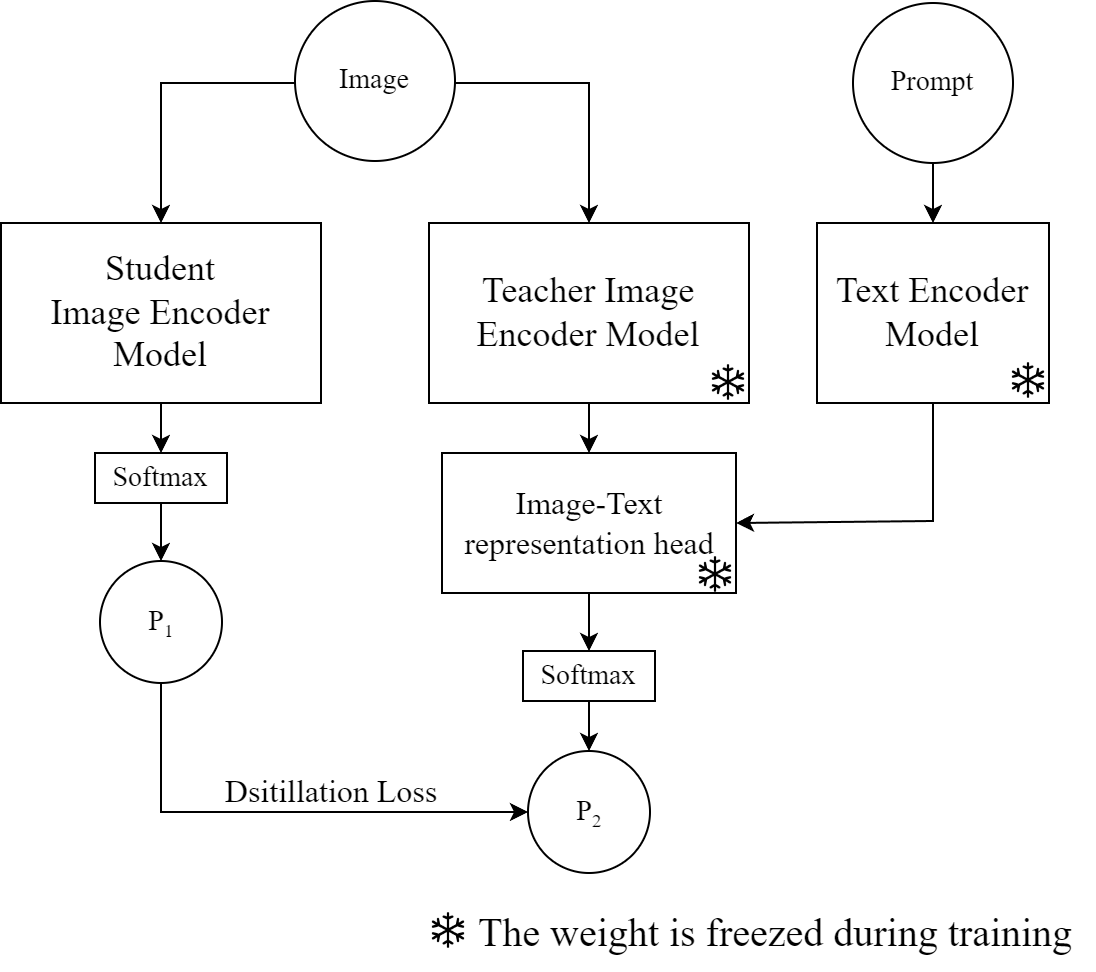
\includegraphics[width=0.8\linewidth]{Images/OverviewMethod.png}
   \end{center}
   \caption{Self-distillation training with image text joined representation.}
   \small
\end{figure}

The result showed that by combining textual information with images, our approach improved accuracy by 3\% in both ResNet \cite{he2016deep} and ViT \cite{dosovitskiy2021an} model compared to the baseline self-distillation method.
The ablation study showed that the student model achieved 3\% higher accuracy by providing detailed descriptions in the training process.
This suggested that by using the text encodings with cross-attention, the model extracted higher semantic information and more precise image representations from the images.
% By repeating our self-distillation method, the accuracy of the student model gradually increases over each repetition.
% Ablation Image-text retrieval

To summarize our contribution.
Firstly this paper investigated the effectiveness of combining text-image representation by using text as a query to emphasize image representation in the self-distillation method.
Secondly, this work proposed a method to efficiently combine textual information and images for the self-distillation method.
Lastly, this work also investigated the effect of prompts in our methods to create image descriptions for training.

\section{Related work}

\subsection{Vision-Language model}

\subsection{Knowledge Distillation and Self-Distillation}

\section{Methodology}

{\small
\bibliographystyle{ieee_fullname}
\bibliography{references}
}

\end{document}
